\documentclass[titlepage]{article}

\usepackage[margin=1in]{geometry}
% some more shit for the title
\usepackage[T1]{fontenc}
\usepackage{babel}

% Tables and stopping them from displaying in a different section
\usepackage{booktabs}
\usepackage[section]{placeins}

% for inserting images into the document, setting file path, and allowing rotation of inserted images 
\usepackage{graphicx}
\graphicspath{ {./images/} }
\usepackage{rotating}
\usepackage[table]{xcolor}
% mostly just for putting text in math equations
\usepackage{amsmath}
% for aligning the text to the left
\usepackage[document]{ragged2e}

% for inserting hyperlinks in the document, use \url{url} or \href{url}{text}
\usepackage{hyperref}
\usepackage{calligra}
\usepackage[T1]{fontenc}
\usepackage{siunitx}
\usepackage{caption}
\usepackage{multirow}
\usepackage[export]{adjustbox}
\usepackage{tikz}
\usepackage{pgfplots}
\pgfplotsset{soldot/.style={color=black,only marks,mark=*},
	             holdot/.style={color=black,fill=white,only marks,mark=*},
		                  compat=1.12}
\usepackage{paracol}

\begin{document}
\title{\textbf{Lab 2: Electric Field and Potential}}
\author{
    Zachary Pouska\\
    \texttt{001103193}\\
    \and
    Natalie Tran \\ 
    \texttt{000698629}\\ \\
} 

\date{PHYS 236 | Fall 2022\\
Date performed: 09/21/2022}


	\maketitle



	\section{Purpose}
	To study the relationship between electric field and the electric potential difference associated with it.
	\section{Theory}	
	The relationship between the electric field and electric potential difference will follow the equation \(\Delta V = -\int_{a}^{b} \vec{E} \cdot ds\), which simplified is \(\Delta V = \frac{k_{e}q}{r}\). This means electric potential will have a opposite yet linear relationship with the electric field, while having an inverse relationship with distance.
	\section{Experiment Analysis}
    
    Using the following equations, we were able to predict many of the results we found during this lab:
    $$\Delta V = -\int_a^b \vec{E}\cdot d\vec{s} $$
    $$V= k_e \int_a^b \frac{dq}{r} $$




	\section{Procedure}
    The experiment is begun by "drawing" the patterns used for the experiments on the conductive surface using conductive ink. This step was performed by our instructor beforehand. 
    \subsection{Perimeter of Conductive Ink and Point Charge}
    The configuration of electrodes below was used for this first part of the experiment. The small circular electrode (white dot) at the center was held at 10 Volts. The green dots indicate where the voltages were measured. 7 points were taking from each side of the positive electrode.

    \FloatBarrier
    \begin{figure}[hbt!]
        \centering
        \caption{Perimeter of conductive ink and point charge setup}
        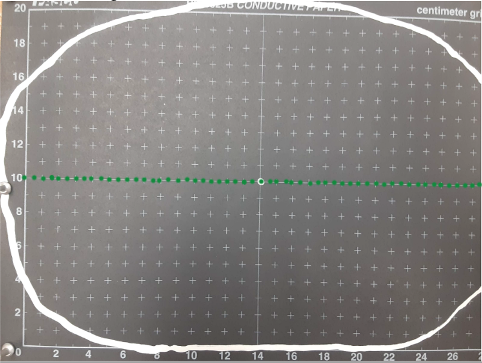
\includegraphics[scale=0.8]{procedure/part1}
    \end{figure} 
    \FloatBarrier



    

    \subsection{Two Point Charges}
    The goal of this experiment was to determine the shape of the equipotential lines resulting from two point charges on a conductive surface. In order to find these equipotential lines, we probed the conductive plate with a digital multimeter, and recorded the results on a piece of graph paper. We measured only four equipotential lines between the two point charges, ranging between 6V and 1.5V. In order to determine the electric field, we use an equation to estimate the magnitude from a potential difference between two points $a$ and $b$.
    $$E=\frac{-V_b-V_a}{\Delta x}$$



    \subsection{Two Plate Capacitor}
    This experiment was similar in nature to the previous one, but just with a different setup. We connected our power supply to the two electrodes of the "capacitor," and begun measuring our equipotential lines. We unfortunately only measured two whole lines, as the setup we received for the lab had the two electrodes very close together. The following is an example of a setup for this lab: 

    \FloatBarrier
    \begin{figure}[hbt!]
        \centering
        \caption{Two Plate Capacitor Setup}
        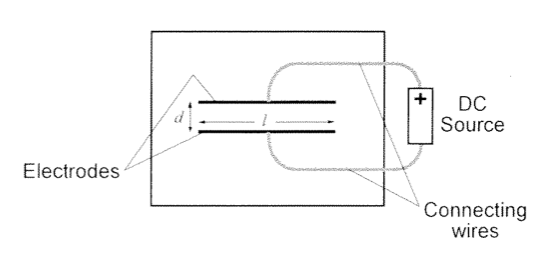
\includegraphics[scale=0.4]{procedure/capacitor}
    \end{figure} 
    \FloatBarrier


    \subsection{One Point and One Line}
    Again, this lab follows a similar set of steps to the previous two. We being by connecting the point charge and line to the power supply leads, and beginning our measurement of the electric potentials. The following figure is another example of the setup for this experiment:

    \FloatBarrier
    \begin{figure}[hbt!]
        \centering
        \caption{Point and Line Example Setup}
        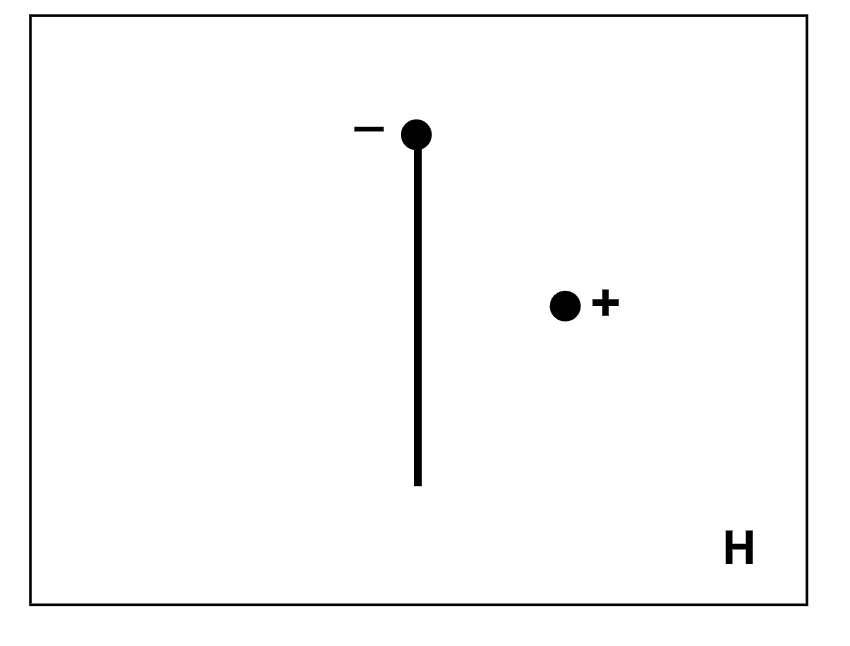
\includegraphics[scale=0.4]{procedure/pointline}
    \end{figure} 
    \FloatBarrier






	\section{Data and Graphs}
	\subsection{Part 1}
	\begin{center}
	\hspace{1.7cm}
	\begin{paracol}{2}
		\begin{table}[h]
		\captionsetup{justification=centering}
		\centering
		\caption*{\textbf{[Table 5.1]} Part 1: Single Point Charge\\ in a 0V Ring\\}
		\rowcolors{2}{gray!10}{gray!40}
		\begin{tabular}{c|c}
			\textbf{Distance (cm)} & \textbf{Voltage (V)}\\
			\hline
			-7 & 1\\
			-6 & 1.1\\
			-5 & 1.3\\
			-4 & 1.3\\
			-3 & 1.5\\
			-2 & 2.3\\
			-1 & 3.7\\
			0 & 9.7\\
			1 & 5.1\\
			2 & 3.9\\
			3 & 3.1\\
			4 & 2.6\\
			5 & 2.2\\
			6 & 1.8\\
			7 & 1.4\\

		\end{tabular}
		\end{table}
	\switchcolumn
	\begin{table}[h]
		\centering
	\caption*{\textbf{[Table 5.1.2]} Table 5.1 With Inversed Voltage}
		\vspace{0.35cm}
		\rowcolors{2}{gray!10}{gray!40}
		\begin{tabular}{c|c}
			\textbf{Distance (cm)} & \textbf{1/Voltage (1/V)}\\
			\hline
			0 & 0.103\\
			1 & 0.196\\
			2 & 0.256\\
			3 & 0.323\\
			4 & 0.385\\
			5 & 0.455\\
			6 & 0.556\\
			7 & 0.714\\
		\end{tabular}
	\end{table}
\end{paracol}
\end{center}
\vspace{1.2cm}
	\begin{center}
		\begin{minipage}[t]{0.45\textwidth}
		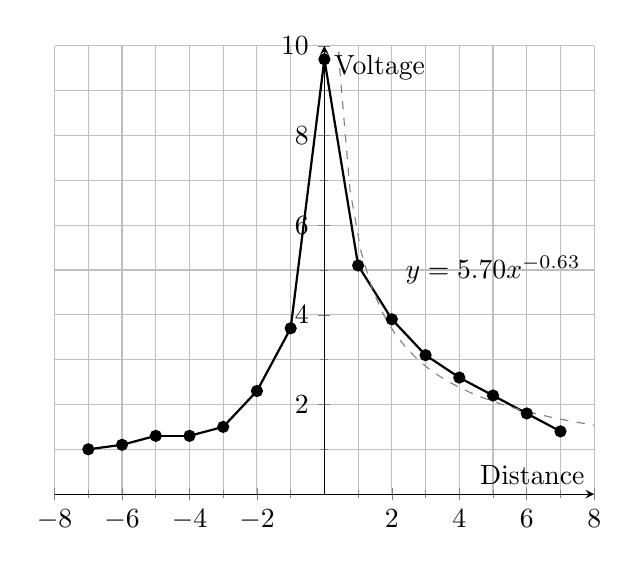
\begin{tikzpicture}
			\begin{axis}[grid=both,
				axis lines=middle,
				xmin=-8,xmax=8,
				ymin=0,ymax=10,
				xtick={-8,-6,-4,-2,0,2,4,6,8},
				ytick={2,4,6,8,10},
				minor tick={-7,-5,-3,-1,1,3,5,7,9},
				xlabel=Distance, ylabel=Voltage]

				\addplot[soldot] coordinates{(-7,1)(-6,1.1)(-5,1.3)(-4,1.3)(-3,1.5)(-2,2.3)(-1,3.7)(0,9.7)(1,5.1)(2,3.9)(3,3.1)(4,2.6)(5,2.2)(6,1.8)(7,1.4)};
			\draw[thick] (-7,1)--(-6,1.1);
			\draw[thick] (-6,1.1)--(-5,1.3);
			\draw[thick] (-5,1.3)--(-4,1.3);
			\draw[thick] (-4,1.3)--(-3,1.5);
			\draw[thick] (-3,1.5)--(-2,2.3);
			\draw[thick] (-2,2.3)--(-1,3.7);
			\draw[thick] (-1,3.7)--(0,9.7);
			\draw[thick] (0,9.7)--(1,5.1);
			\draw[thick] (1,5.1)--(2,3.9);
			\draw[thick] (2,3.9)--(3,3.1);
			\draw[thick] (3,3.1)--(4,2.6);
			\draw[thick] (4,2.6)--(5,2.2);
			\draw[thick] (5,2.2)--(6,1.8);
			\draw[thick] (6,1.8)--(7,1.4);
			\addplot[domain=0.1:8,dashed,gray] {5.7*x^(-0.63)};
			\node at (5,5) {$y = 5.70x^{-0.63}$};
			\end{axis}
		\end{tikzpicture}
		\centering
		\textbf{[Fig 5.1]} Table 5.1 visualized in a graph.
		\end{minipage}
		\hspace{1cm}
		\begin{minipage}[t]{0.45\textwidth}
		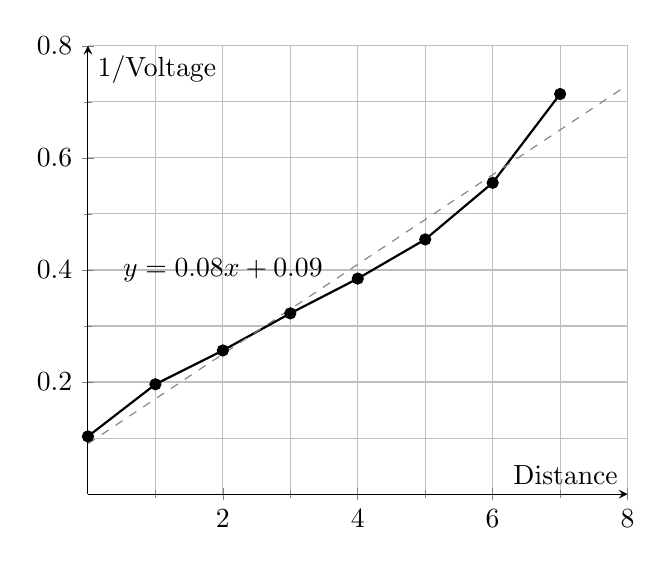
\begin{tikzpicture}
			\begin{axis}[grid=both,
				axis lines=middle,
				xmin=0,xmax=8,
				ymin=0,ymax=0.8,
				xtick={0,2,4,6,8},
				ytick={0,0.2,0.4,0.6,0.8},
				minor y tick num=1,
				minor x tick num=1,
				xlabel={Distance}, ylabel={1/Voltage}]

				\addplot[soldot] coordinates{(0,0.103)(1,0.196)(2,0.2564)(3,0.32258)(4,0.3846)(5,0.4545)(6,0.55555)(7,0.714)};
				\draw[thick] (0,0.103)--(1,0.196); 
				\draw[thick] (1,0.196)--(2,0.2564); 
				\draw[thick] (2,0.2564)--(3,0.32258); 
				\draw[thick] (3,0.32258)--(4,0.3846); 
				\draw[thick] (4,0.3846)--(5,0.4545); 
				\draw[thick] (5,0.4545)--(6,0.55555); 
				\draw[thick] (6,0.55555)--(7,0.714); 
				\addplot[domain=0:8,dashed,gray] {0.08*x+0.09};
				\node at (2,0.4) {$y = 0.08x+0.09$};
			\end{axis}
		\end{tikzpicture}
		\centering
		\textbf{[Fig 5.1.2]} The linearization of Fig 5.1.
	\end{minipage}
	\end{center}
	\vspace{3cm}
	\subsection{Part 2} 
	\vspace{0.7cm}
	\begin{paracol}{2}
		\begin{minipage}[t]{0.5\textwidth}
			\centering
			[\textbf{Fig 5.2}] Part 2: Two Point Charges
			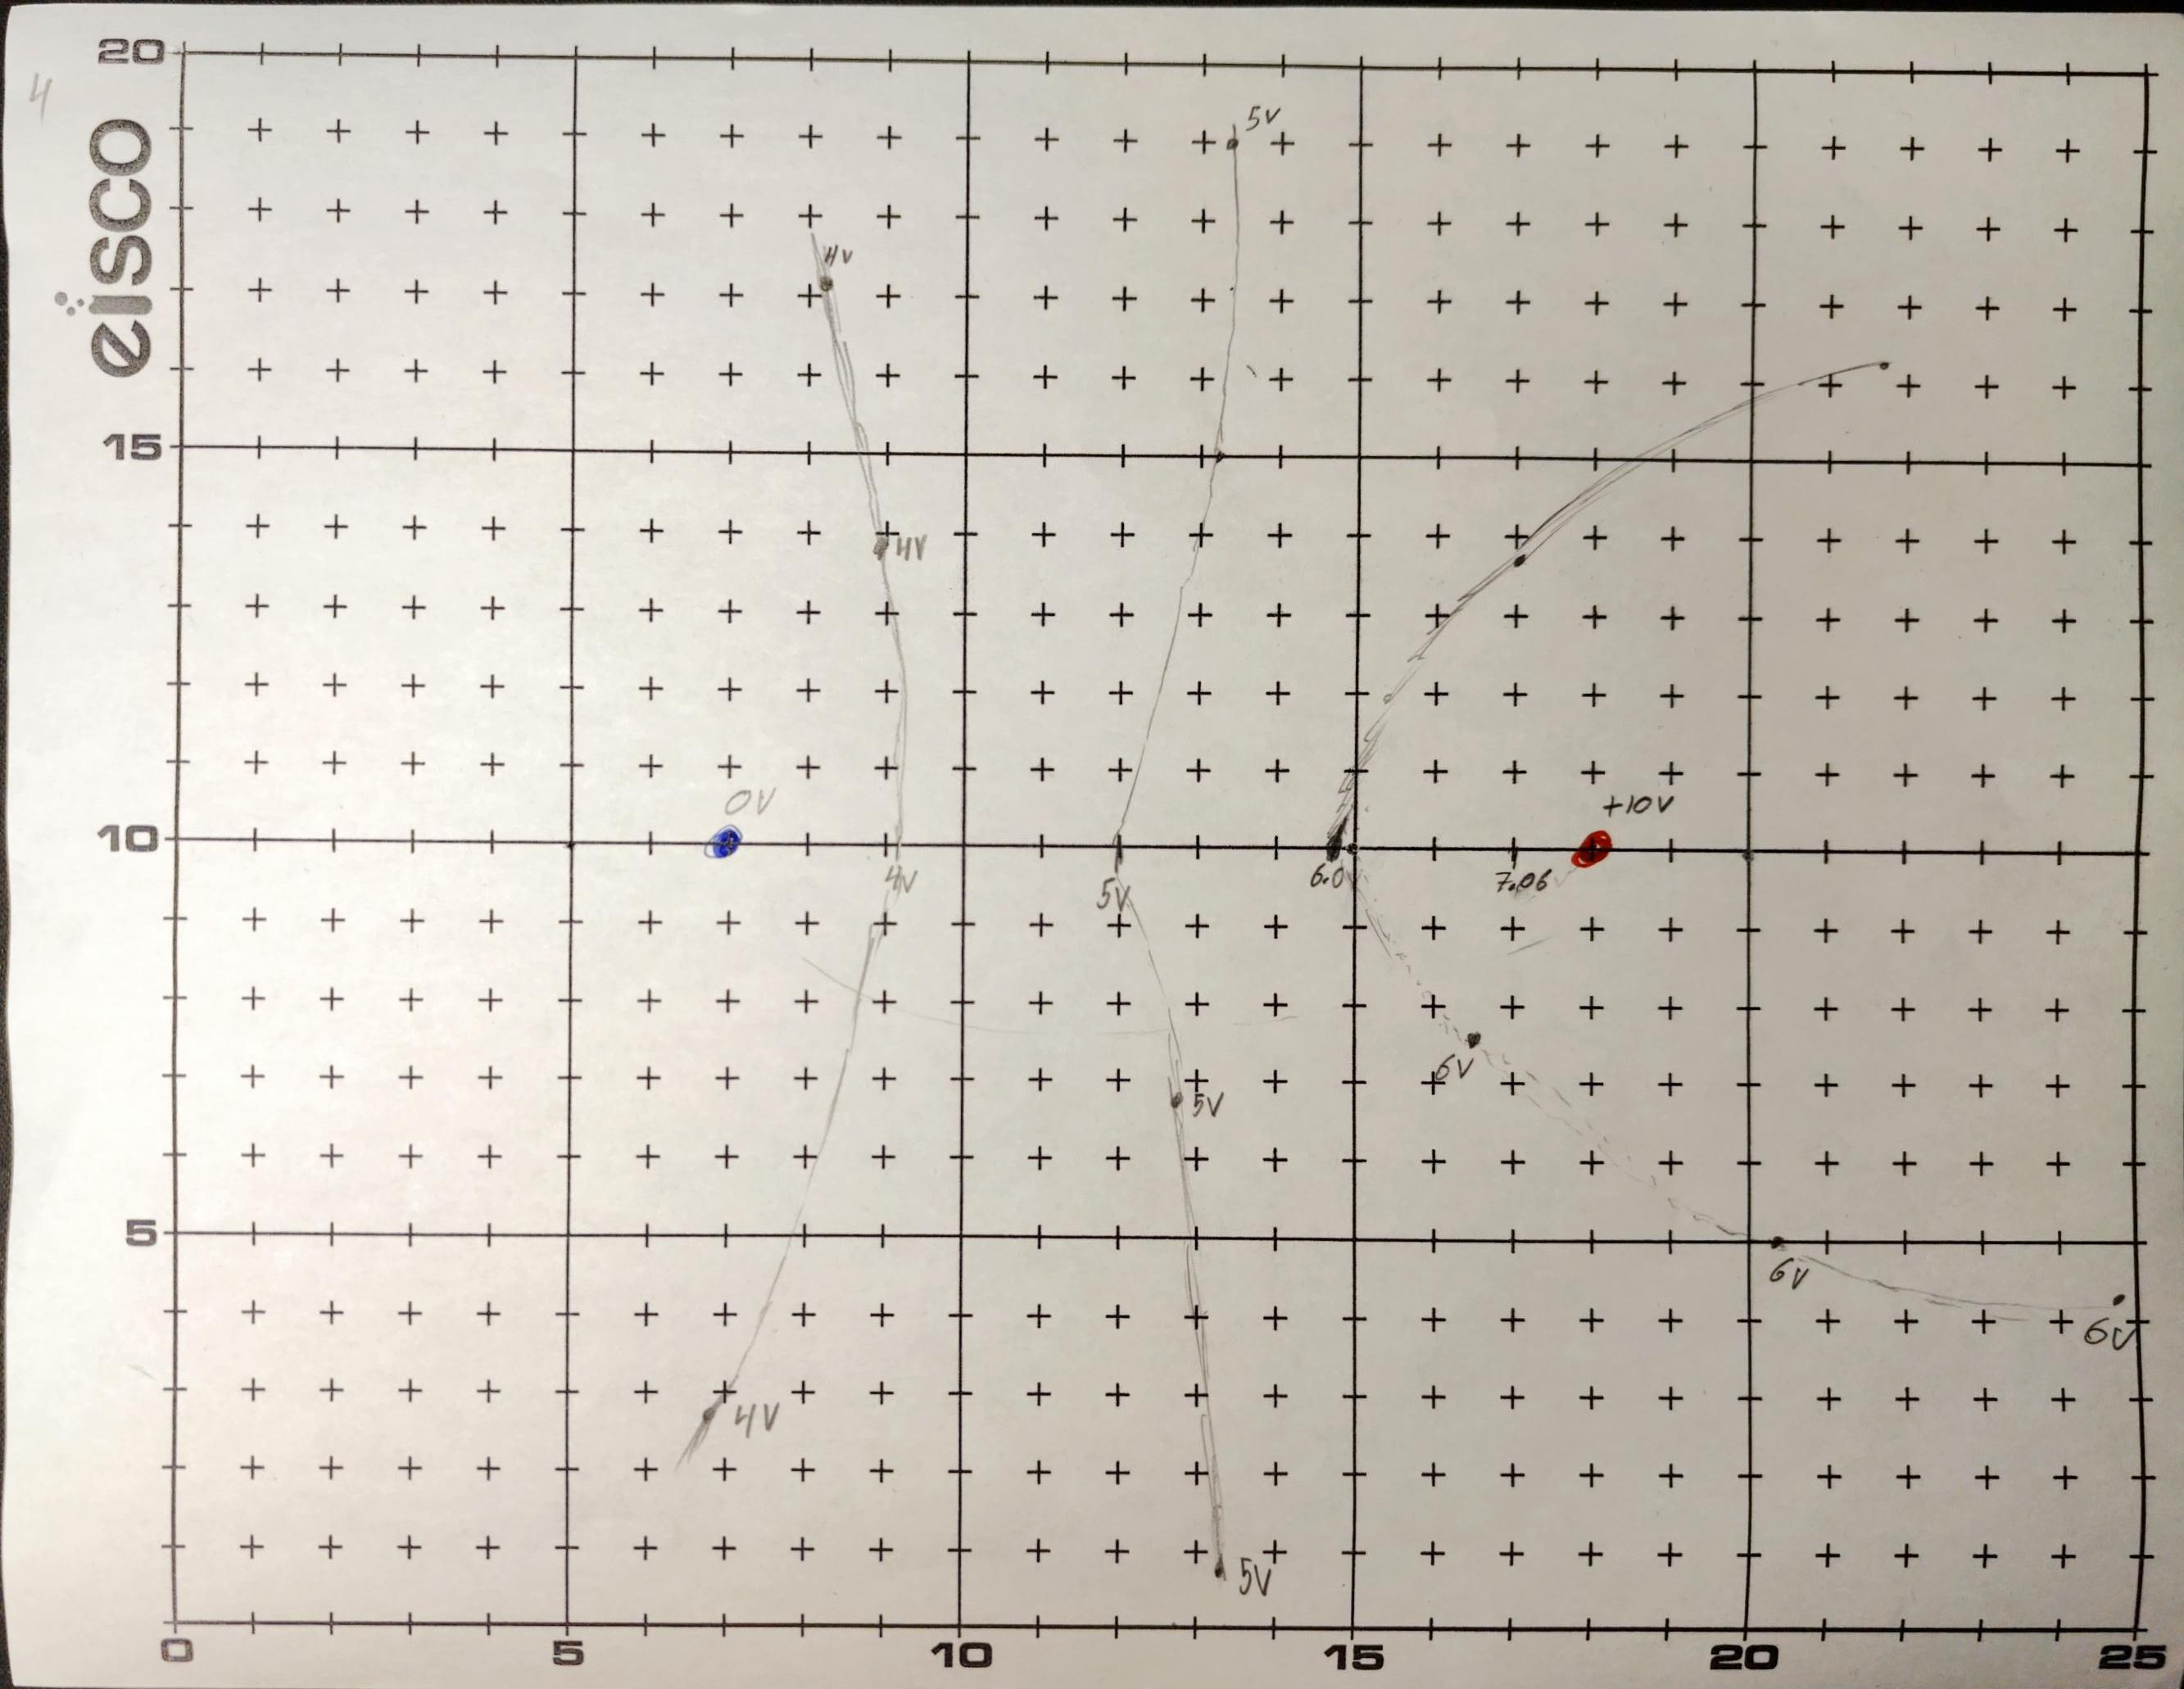
\includegraphics[width=1\linewidth, frame]{part2}
		\end{minipage}
		\switchcolumn
		\begin{minipage}[c]{0.5\textwidth}
			\vspace{1.7cm}
			\begin{center}
			[\textbf{Table 5.2}] Fig 5.2 Analyzed
		\end{center}
		\rowcolors{3}{gray!10}{gray!40}
			\begin{tabular}{c|c|c}
				\textbf{Distance between} & \textbf{Voltage} & \textbf{Electric Field} \\
				\textbf{Equipotentials} & \textbf{Difference (V)} & \textbf{Magnitude (V/m)}\\
				\hline
				2.8 cm & 1 & 35.7\\
				2.8 cm & 1 & 35.7
			\end{tabular}
		\end{minipage}
	\end{paracol}
	\vspace{3cm}
	\subsection{Part 3}
	\begin{center}
			[\textbf{Fig 5.3}] Part 3: Two Line Charges	
	\end{center}
		\begin{center}
			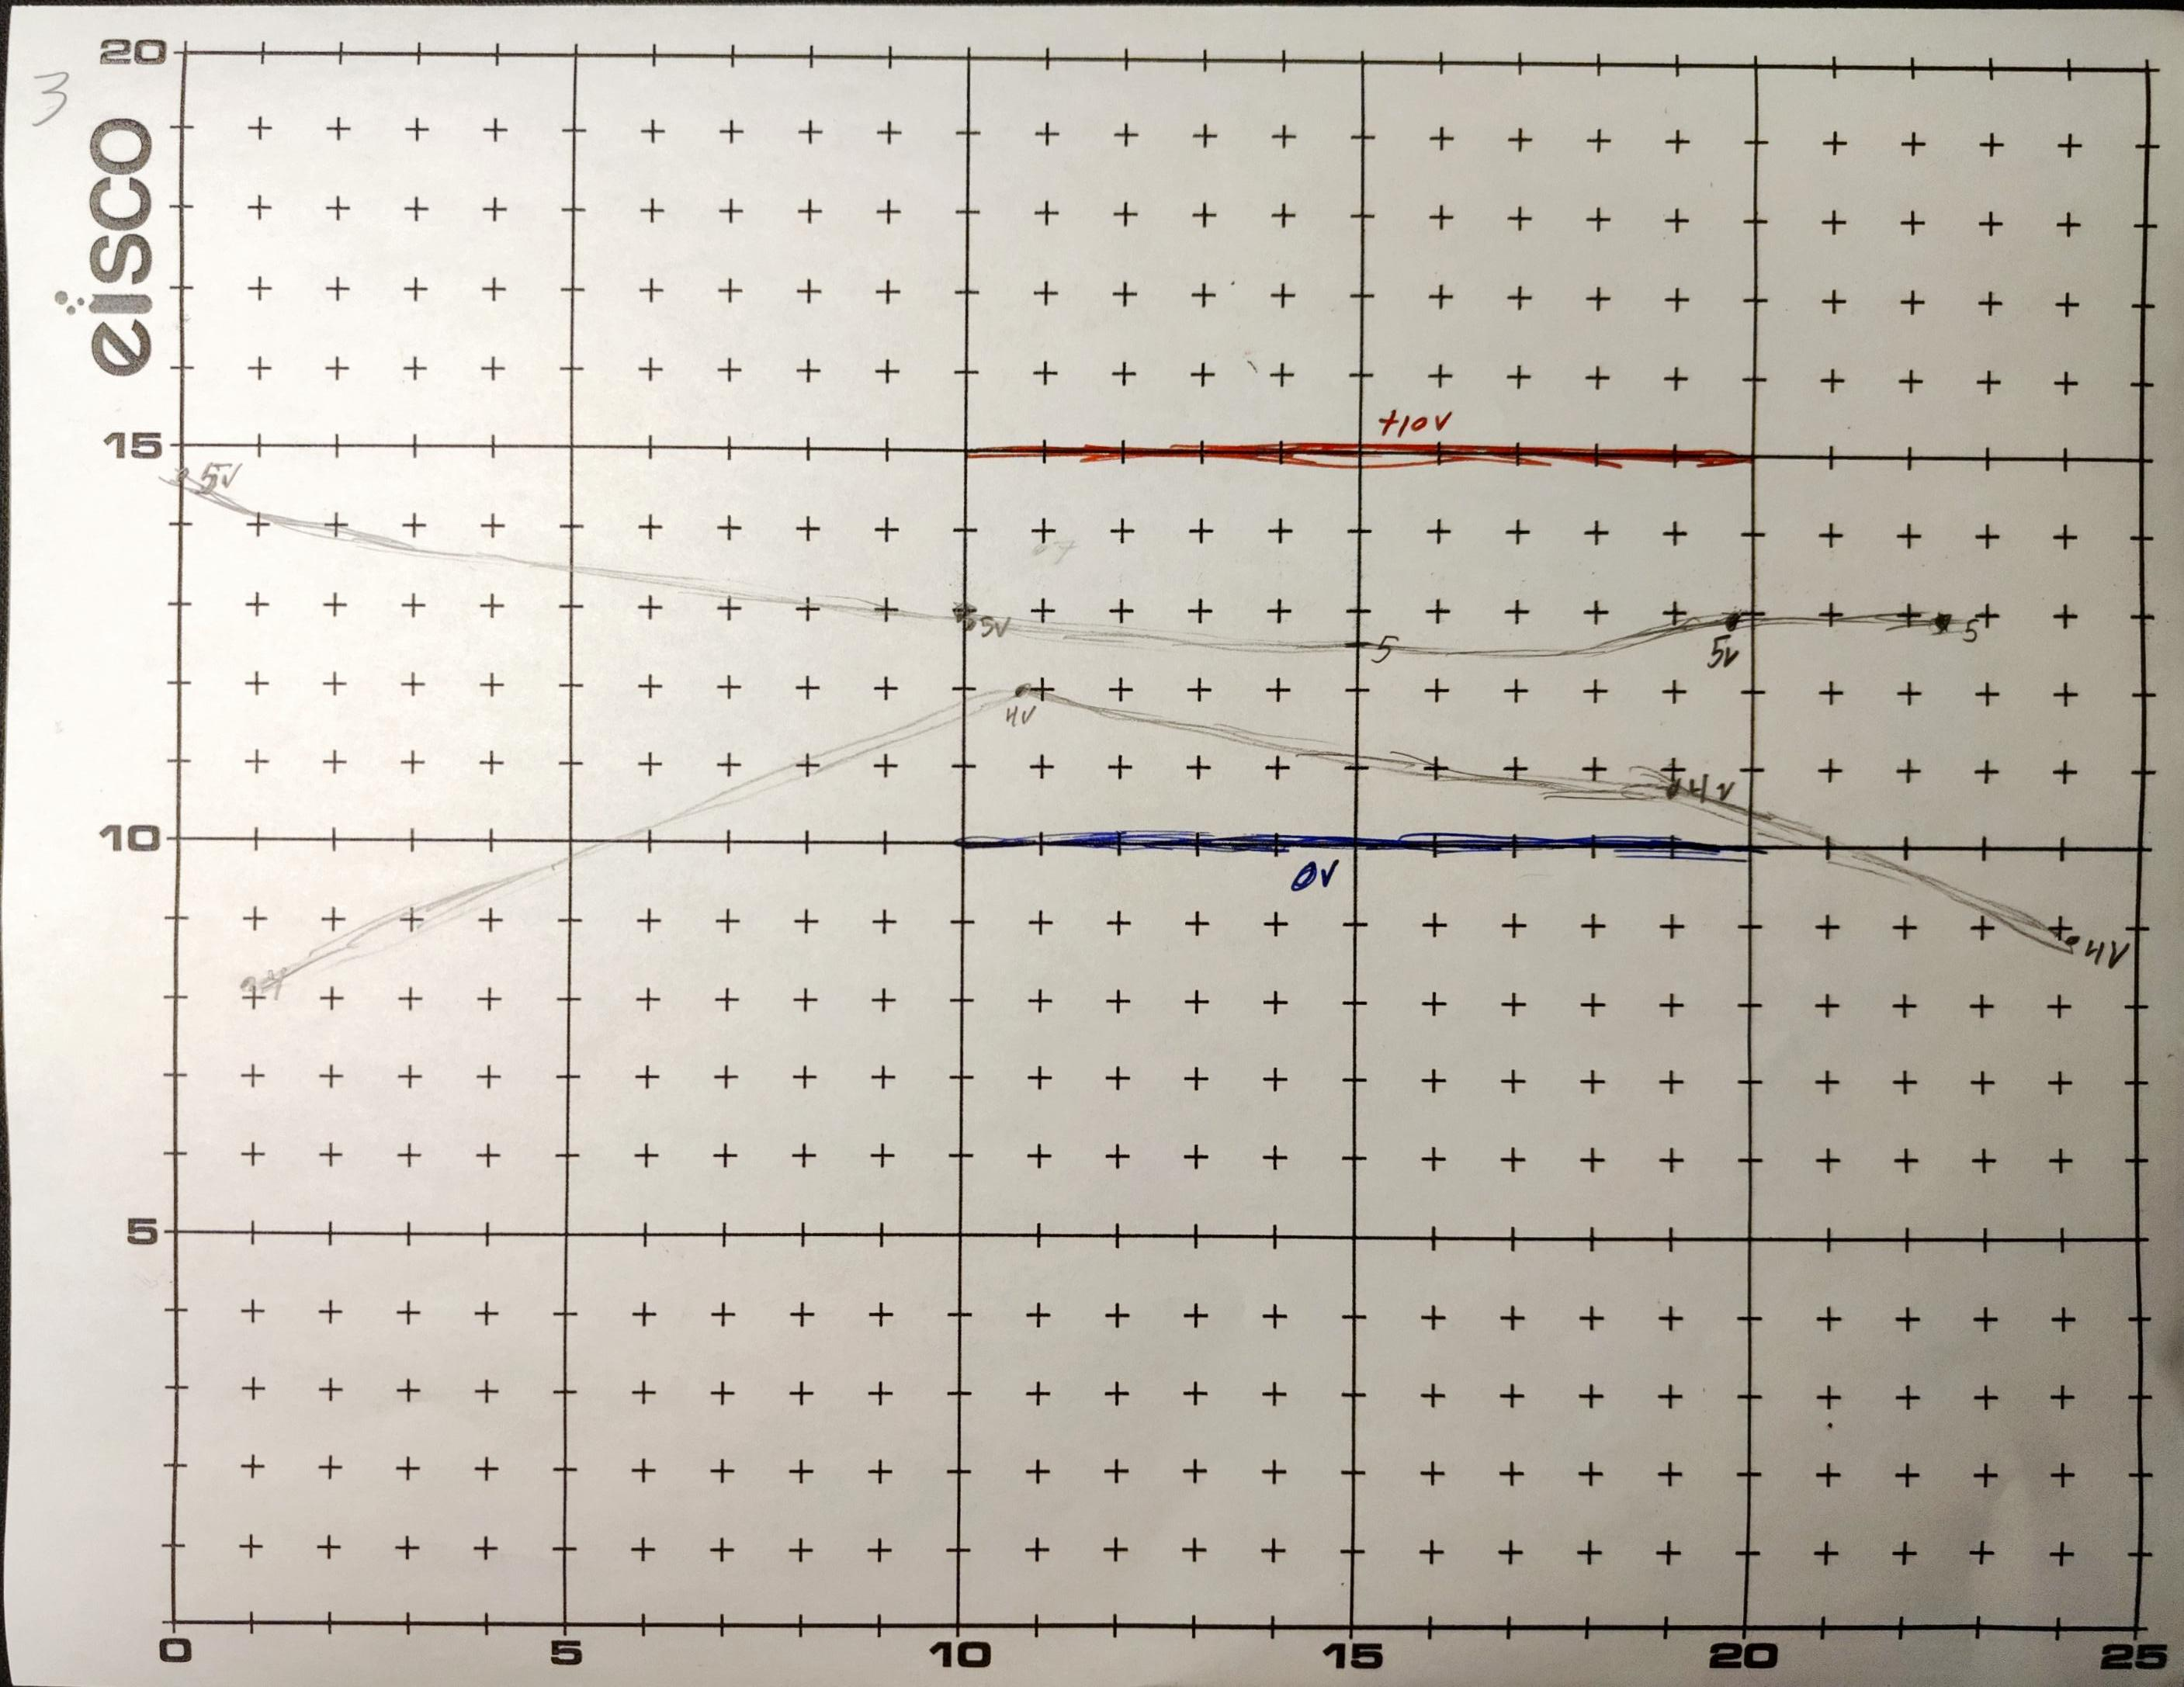
\includegraphics[width=0.5\linewidth, frame]{part3}
		\end{center}
`	\subsection{Part 4}
		\begin{center}
			[\textbf{Fig 5.4}] Part 4: One Line Charge and One Point Charge	
		\end{center}

		\begin{center}
			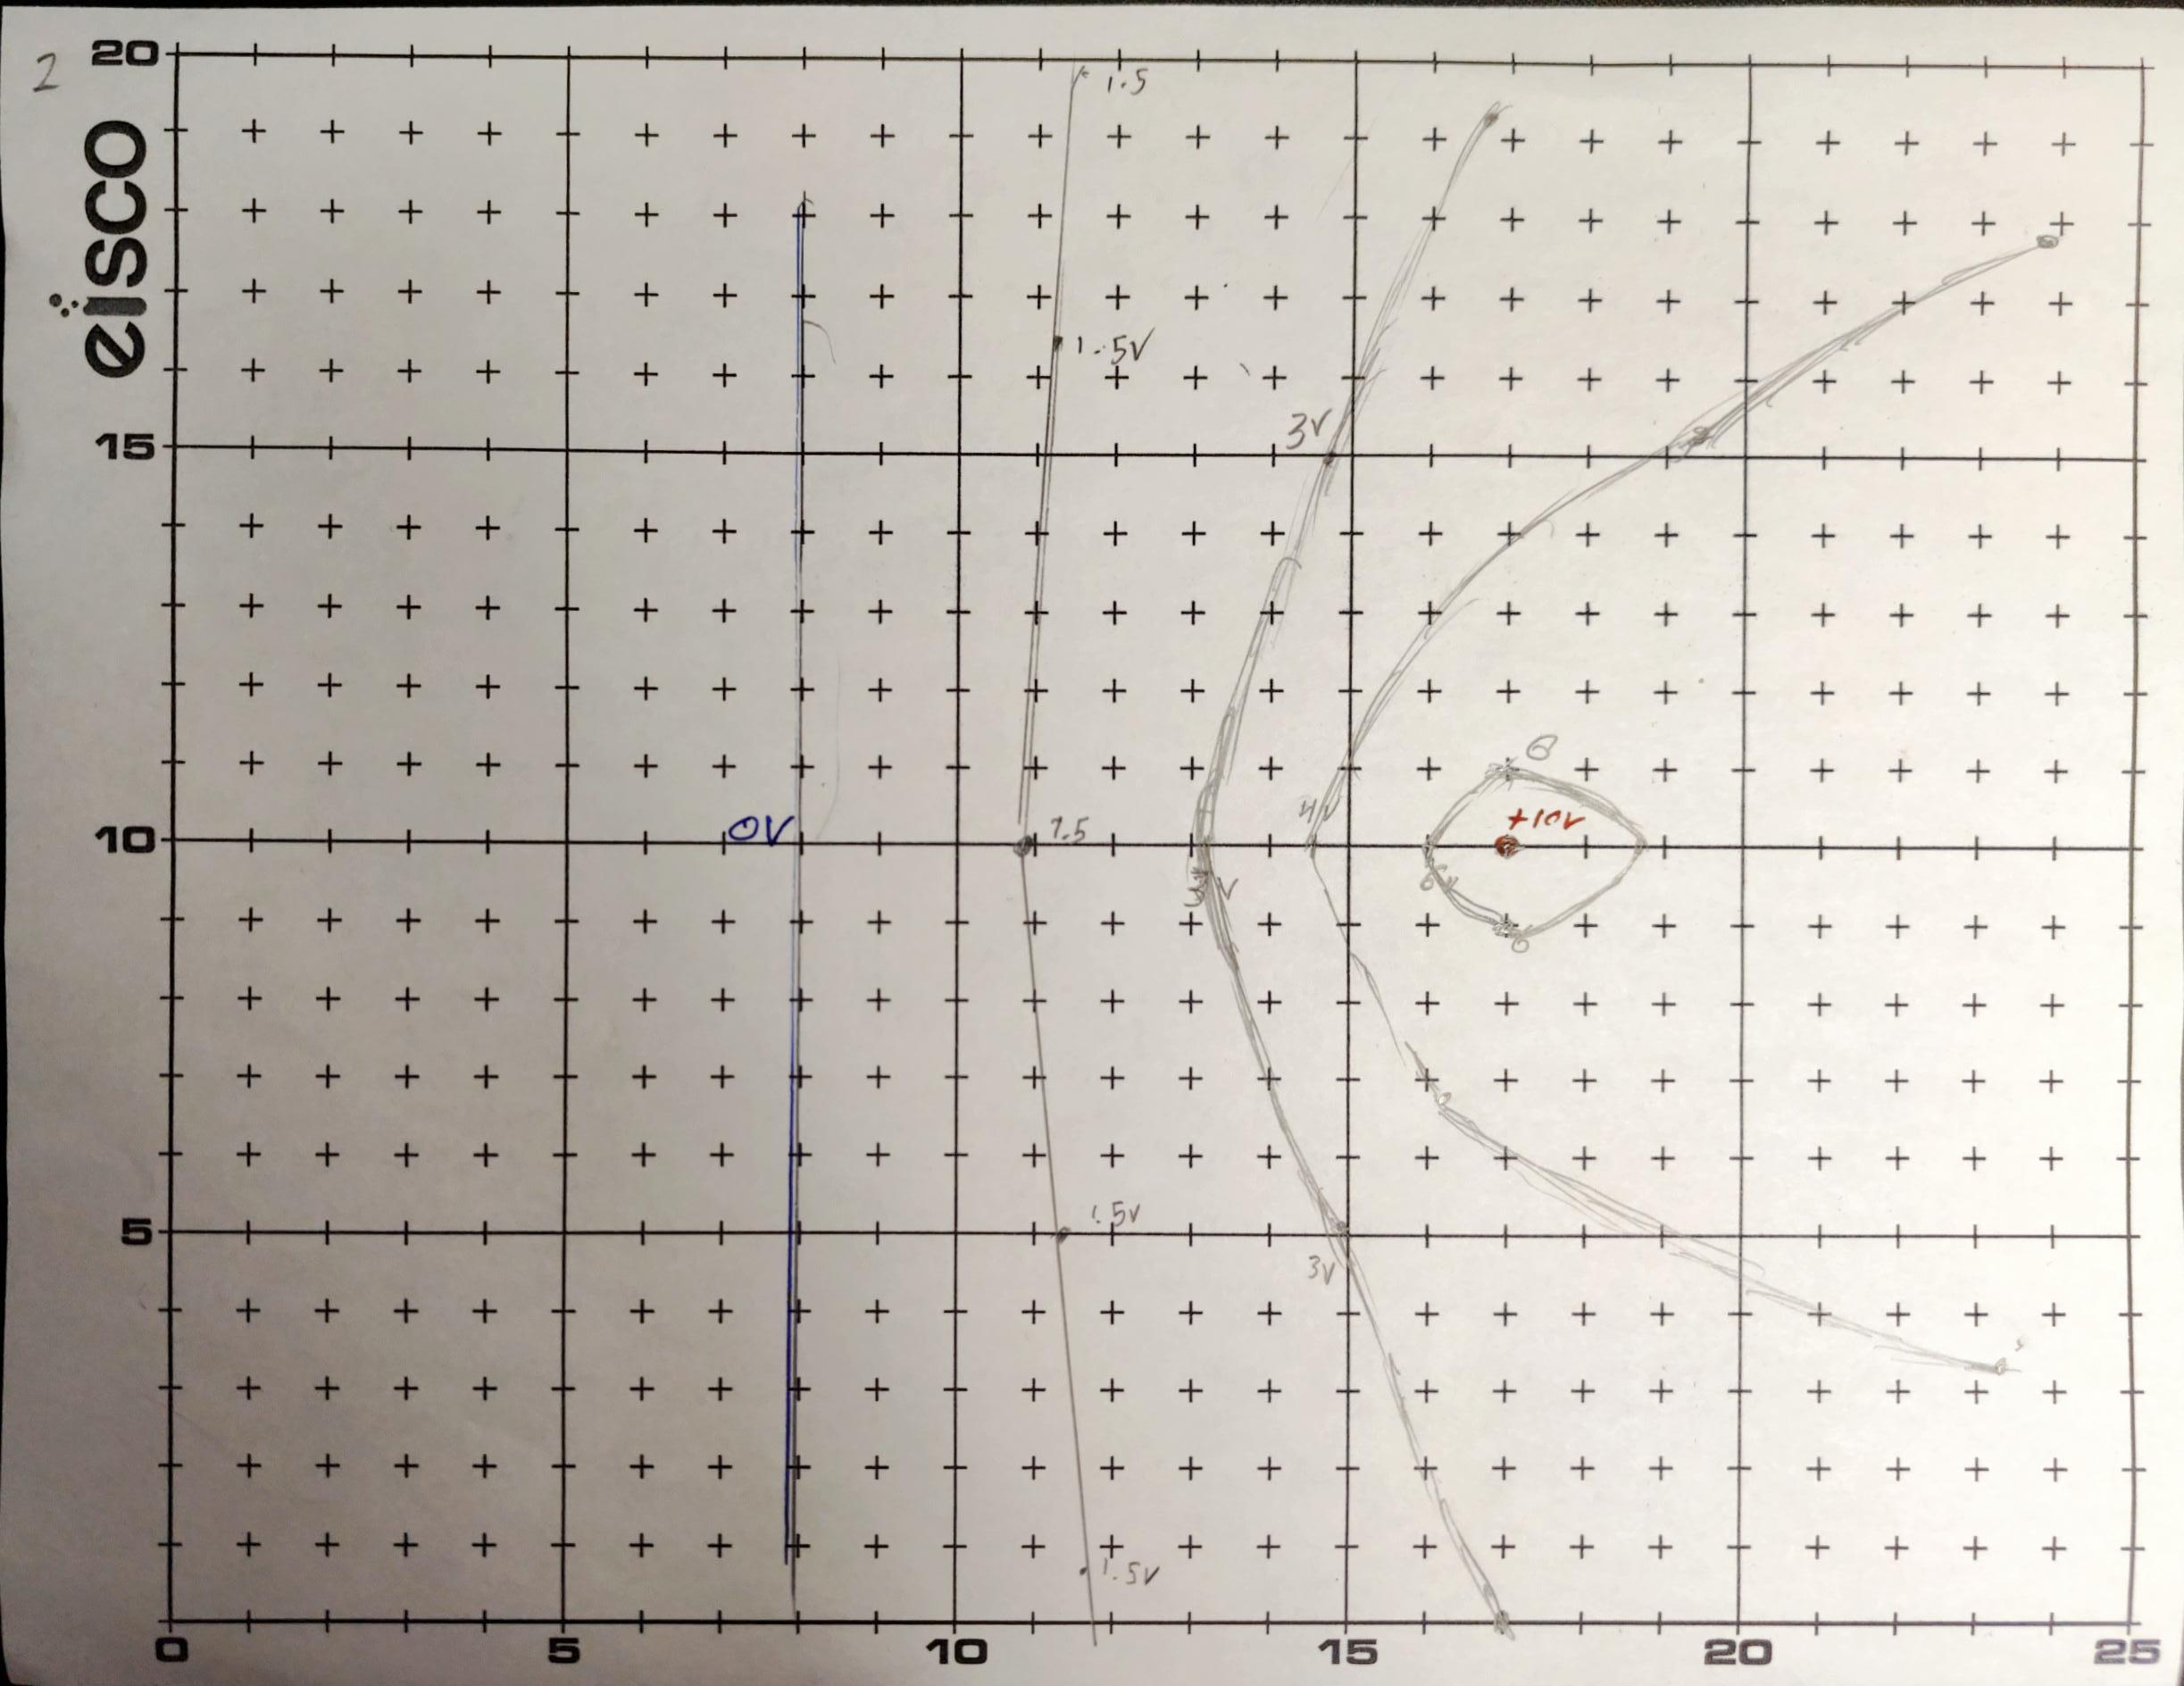
\includegraphics[width=0.5\linewidth, frame]{part4}
		\end{center}
	\section{Results}
    Using the following equations, we were able to predict many of the results we found during this lab:
    $$\Delta V = -\int_a^b \vec{E}\cdot d\vec{s} $$
    $$V= k_e \int_a^b \frac{dq}{r} $$

		\begin{minipage}[t]{0.4\textwidth}
            \centering
		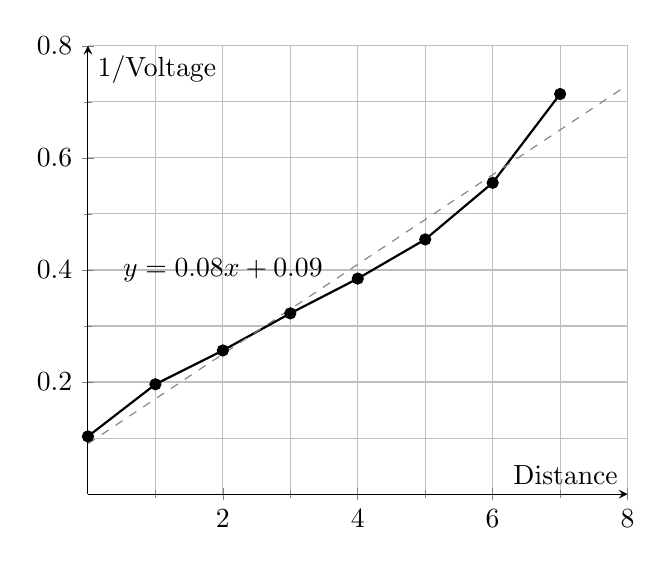
\begin{tikzpicture}
			\begin{axis}[grid=both,
				axis lines=middle,
				xmin=0,xmax=8,
				ymin=0,ymax=0.8,
				xtick={0,2,4,6,8},
				ytick={0,0.2,0.4,0.6,0.8},
				minor y tick num=1,
				minor x tick num=1,
				xlabel={Distance}, ylabel={1/Voltage}]

				\addplot[soldot] coordinates{(0,0.103)(1,0.196)(2,0.2564)(3,0.32258)(4,0.3846)(5,0.4545)(6,0.55555)(7,0.714)};
				\draw[thick] (0,0.103)--(1,0.196); 
				\draw[thick] (1,0.196)--(2,0.2564); 
				\draw[thick] (2,0.2564)--(3,0.32258); 
				\draw[thick] (3,0.32258)--(4,0.3846); 
				\draw[thick] (4,0.3846)--(5,0.4545); 
				\draw[thick] (5,0.4545)--(6,0.55555); 
				\draw[thick] (6,0.55555)--(7,0.714); 
				\addplot[domain=0:8,dashed,gray] {0.08*x+0.09};
				\node at (2,0.4) {$y = 0.08x+0.09$};
			\end{axis}
		\end{tikzpicture}
		[Fig 1.2] The linearization of Fig 1.1.
	\end{minipage}

	\section{Questions}
	\subsection{Part 1}
		\begin{enumerate}
			\item Which function will describe the behavior?\\
				An inverse function.
			\item Fit it with the best fit line. What does the coefficient in the equation given by excel mean?\\
				The coefficient of the equation represents the electric field.
			\item Paste your graph with fitting line here.\\
				See Fig 5.1.
		\end{enumerate}
		\vspace{5cm}
	\subsection{Part 2}
		\begin{enumerate}
			\item \textbf{Choose two equipotential points and calculate the electric field}\\
				See Table 5.2
            \item \textbf{Include a picture of your equipotential lines for this configuration here. With a pen or marker of different color draw the electric field lines.}\\
				See Fig 5.2
            \item \textbf{Do equipotential lines cross? Why or why not?}\\
				They do not cross because they are lines of constant potential. There cannot be a point of 2 different potentials in an equipotential line.
            \item \textbf{Which direction does the electric field point with respect to equipotential? Does E point to high or low electric potential?}\\
				It goes from high to low electric potential.
            \item \textbf{In this final step we will combine the direction information given by the equipotentials with the magnitude information from the measured potential differences discussed above. First estimate the magnitude and record your results in this chart.}\\
				See Table 5.2.
		\end{enumerate}
		\subsection{Part 3}
		\begin{enumerate}
			\item Given the voltage difference between the two plates and the separation distance what is the magnitude of the electric field inside the plates? Do this calculation using at last three combinations of equipotential lines.\\
		\begin{center}
				\begin{table}[h]
		\rowcolors{3}{gray!10}{gray!40}
			\begin{tabular}{c|c|c}
				\textbf{Distance between} & \textbf{Voltage} & \textbf{Electric Field} \\
				\textbf{Equipotentials} & \textbf{Difference (V)} & \textbf{Magnitude (V/m)}\\
				\hline
				1.6 cm & 1 & 62.5\\
			\end{tabular}
		\end{table}
	\end{center}

			\item Include a photo of the equipotential lines and the electric field that you found for this configuration.\\
				See Fig 5.3.
		\end{enumerate}
		\subsection{Part 4}
		\begin{enumerate}
			\item What is the magnitude of the electric field inside the "plates"?\\
				\FloatBarrier
				\begin{center}
				\begin{table}[hbt!]
		\rowcolors{3}{gray!10}{gray!40}
			\begin{tabular}{c|c|c}
				\textbf{Distance between} & \textbf{Voltage} & \textbf{Electric Field} \\
				\textbf{Equipotentials} & \textbf{Difference (V)} & \textbf{Magnitude (V/m)}\\
				\hline
				1.5 cm & 2 & 133\\
				1.4 cm & 1 & 71.4    \\
				2.0 cm & 1.5 & 75  \\
			\end{tabular}
			\end{table}
			\end{center}
			\FloatBarrier
			\item Include a photo of the equipotential lines and the electric field that you found for this configuration.\\
			See Fig 5.4.
		\end{enumerate}
	\section{Conclusion}
    Overall, this lab was successful in empirically verifying the concepts learned throughout the last chapter of this class, and further familiarizing us with the electronics lab equipment. There were unfortunately a few cases where our group did not take as many data points as were originally instructed, but overall our data appears to have a relatively low error rate. Probably one of the main sources of error in this lab would be the setup of the conductive paint on the plates. The paint was not very consistently applied from point to point, probably causing a bit of variation in the electric field throughout the plate. 
\end{document}
